% The superblock of two-site DMRG: the effective Hamiltonian the eigensolver is
% handed at one step of a sweep.
%
% It is the fixed point's left-hand side with the state removed. Take L from
% 07 -- the tall tensor carrying one index into each layer and one into the
% Hamiltonian -- take A and its conjugate out of the column, and what is left is
% L with its bra and ket indices free. Put that on the left, its mirror on the
% right, the two MPO tensors of the sites being optimised between them, and the
% picture is H_eff.
%
% Every free index ends where the absent tensor's own leg would be, which is the
% only way the gap is a gap and not just white space. The two-site tensor Theta
% is a box of height \tnThetaH whose centre sits at \tnThetaY: so the bond
% indices leave L and R horizontally at that centre height, and the physical
% indices of W stop at its near edge, half that height short. They are
% deliberately not all at one depth -- a tensor's bond legs and its physical
% legs do not leave it at one height either, and lining them up would mean they
% no longer point at anything.
%
% Theta's bond spans the gap the row already has, so the stubs are exactly that
% gap long. \tnrow sets the gap once and places everything from it; the row
% holds two shapes of different widths and heights and none of their positions
% is worked out by hand.
%
% The gaps are left empty on purpose: drawing Theta in would make this a picture
% of one application rather than of the operator.
\documentclass[border=4pt]{standalone}
\usepackage{amsmath,amssymb}
\usepackage{tikz-tensors}

\def\tnGap{6mm}      % between neighbours in the row, and so Theta's bond
\def\tnThetaY{1.35}  % where Theta's centre sits, above and below
\def\tnThetaH{0.45}  % half its height: where its near edge is

\tikzset{env/.style={tn node, minimum width=7mm, minimum height=31mm}}
\begin{document}
\begin{tikzpicture}
  \tnrow[\tnGap]{P}{(0,0)}{env/$L$/c, mpo/$W$/c, mpo/$W$/c, env/$R$/c}
  \foreach \i [evaluate=\i as \j using int(\i+1)] in {1,2,3}{
    \tnbond[disc]{(P\i) -- (P\j)}%
  }

  \foreach \s/\p in {1/{'}, -1/{}} {
    % the bond indices, at the height of Theta's own, and as long as its bond
    \tnbond[disc]{([yshift=\s*\tnThetaY cm]P1.east) -- ++(\tnGap,0)}
    \tnbond[disc]{([yshift=\s*\tnThetaY cm]P4.west) -- ++(-\tnGap,0)}
    % the physical indices, stopping at Theta's near edge
    \tnbond[disc]{(P2) -- (P2 |- 0,\s*\tnThetaY-\s*\tnThetaH)}
    \tnbond[disc]{(P3) -- (P3 |- 0,\s*\tnThetaY-\s*\tnThetaH)}
  }
  \tnput[above]{[yshift=\tnThetaY cm,xshift=\tnGap]P1.east}{$a'$}
  \tnput[above]{P2 |- 0,\tnThetaY-\tnThetaH}{$\sigma_1'$}
  \tnput[above]{P3 |- 0,\tnThetaY-\tnThetaH}{$\sigma_2'$}
  \tnput[above]{[yshift=\tnThetaY cm,xshift=-\tnGap]P4.west}{$b'$}
  \tnput[below]{[yshift=-\tnThetaY cm,xshift=\tnGap]P1.east}{$a$}
  \tnput[below]{P2 |- 0,-\tnThetaY+\tnThetaH}{$\sigma_1$}
  \tnput[below]{P3 |- 0,-\tnThetaY+\tnThetaH}{$\sigma_2$}
  \tnput[below]{[yshift=-\tnThetaY cm,xshift=-\tnGap]P4.west}{$b$}
\end{tikzpicture}
\end{document}
